% F25 The five-panel video comparison (man_walking.mp4). Added 6 Nov.
% Image: the video embedded on slide 18 of the author's final presentation (5 Nov; ppt/media/media1.mp4, 3360 x 736,
% 356 frames, 29.97 FPS); frame 178 extracted with ffmpeg (the slide's poster frame, ppt/media/image18.png, is frame 0),
% black letterbox bars cut, the five 672-px panels rearranged 2 + 2 + 1 (scratchpad script make_images.py); nothing
% else changed: titles and FPS labels are the ones burned into the video. Saved as figures/img/F25_video_panels.jpg
% (1356 px wide, JPEG quality 85). FPS values: numbers_nov.tex \Video...FPS; confirmed against timing.csv of job 3657550 (7 Nov).
\begin{figure}[!tbp]
\centering
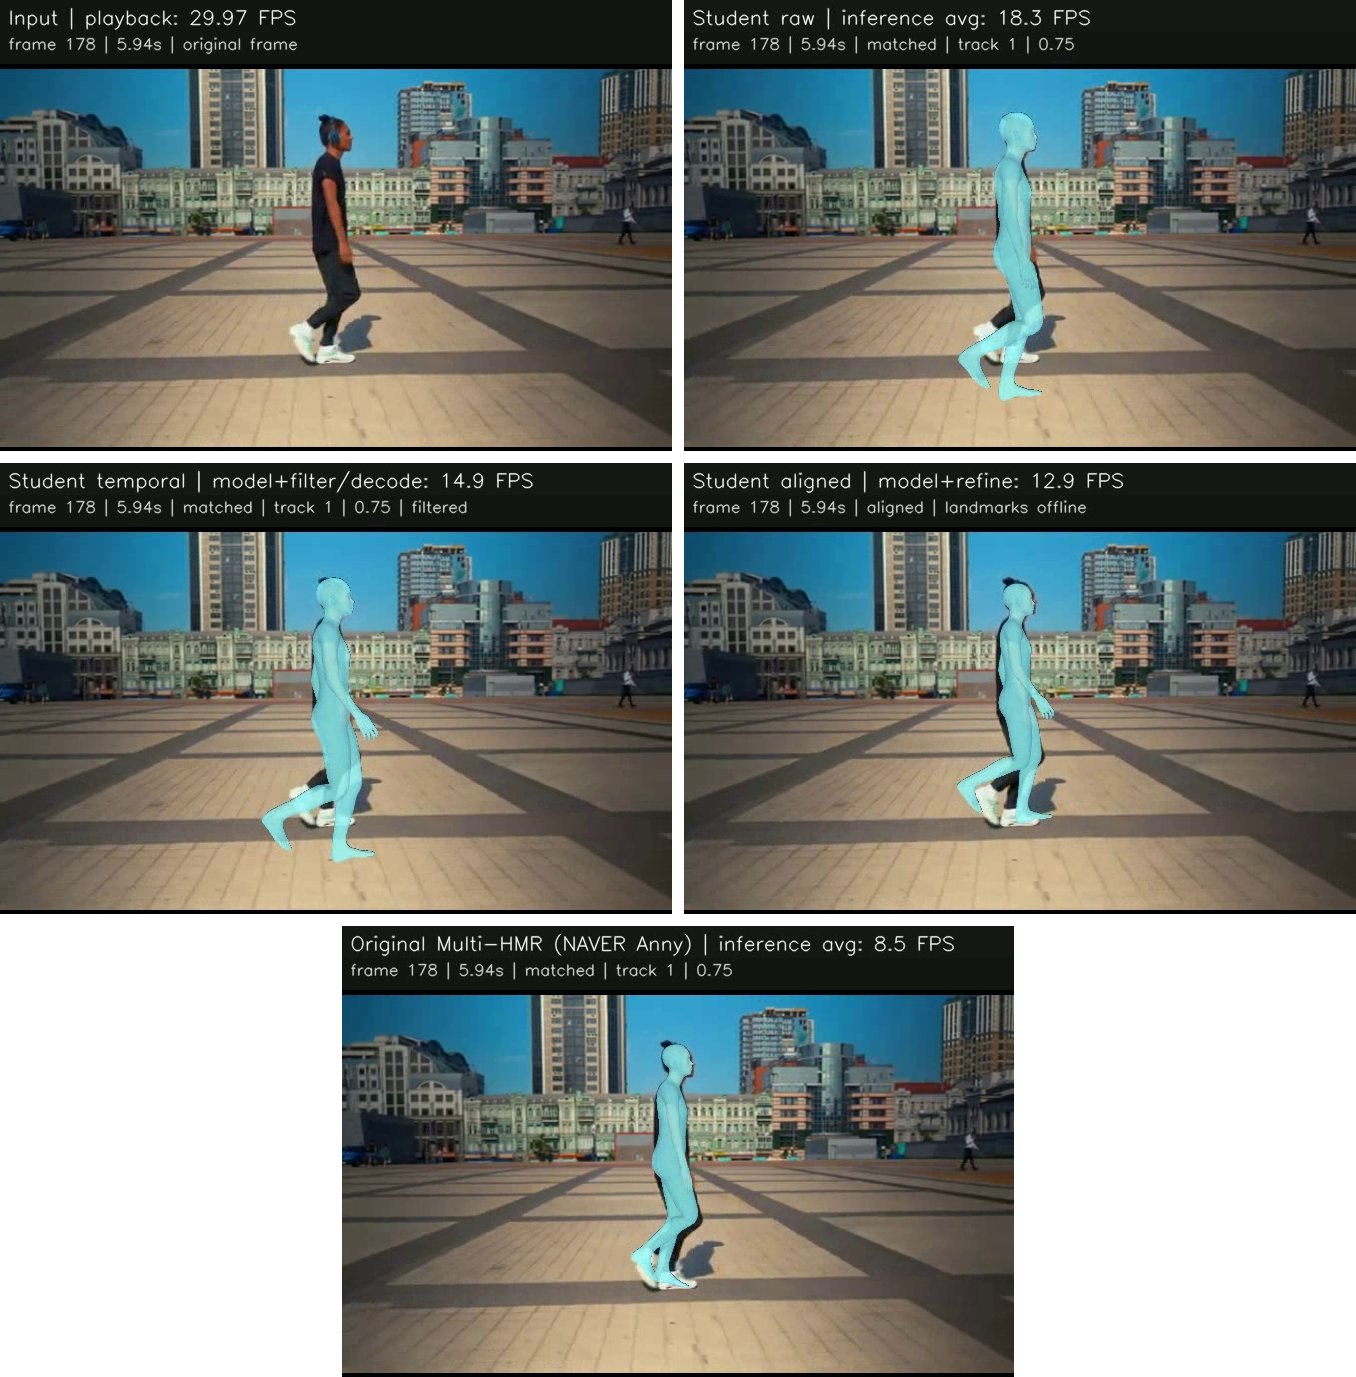
\includegraphics[width=\linewidth]{F25_video_panels.jpg}
\caption[Video comparison: student variants and the released baseline]{Frame \VideoFigureFrame{} of
\VideoFrames{} of the walking clip: input (top left), raw student (top right), student with temporal filtering
(``Student temporal'', middle left), student with landmark alignment (``Student aligned'', middle right) and the
released baseline (``Original Multi-HMR (NAVER Anny)'', bottom). The FPS printed in each panel (playback for the
input, model inference for the raw panels, model plus filter or alignment for the others) excludes preprocessing,
landmark extraction and video input and output (Table~\ref{tab:video-fps}).}
\label{fig:video-panels}
\end{figure}
